\documentclass[fleqn]{jbook}
\usepackage{physpub}

\begin{document}

\begin{question}{教育 物理}{}


\begin{subquestions}
\SubQuestion
  地球からロケットを発射する。ただしロケットは発射時のごく短い時間
  だけ噴射するものとし、飛行中のロケットの質量 $m$ は地球の質量 $M$
  より十分に小さく、かつ一定であるとする。またロケットは質点とみなし、
  かつ球対称な重力場の中を運動するものとして、空気の抵抗は無視する。
  地球の中心からロケットまでの距離を $r$ として、以下の問いに答えよ。
  ただし、数値は有効数字2けたまで計算するものとし、以下の数値を用いて
  よい。
%
  \begin{quote}
    重力定数   $G=6.67\Keta{-11}\Unit{Nm^2kg^{-2}}$ \\
    地球の質量 $M=5.97\Keta{24} \Unit{kg}$ \\
    地球の半径 $R=6.38\Keta{6}\Unit{m}$
  \end{quote}

  \begin{subsubquestions}
  \SubSubQuestion
    2次元の極座標 $(r,\theta)$ においてロケットに働く力の成分を
    $(F_r,F_\theta)$ とすると、ロケットの運動方程式は、
%
    \[ F_r = m \Bigl[%
              \Deriver{^2r}{t^2} - r \Bigl(\Deriver{\theta}{t}\Bigr)^2%
             \Bigr]  \hspace{15mm}%
       F_{\theta} = \frac{m}{r}\Deriver{}{t}\Bigl(%
              r^2\Deriver{\theta}{t}%
             \Bigr) \]
%
    のように書ける。いまの設問の場合、角運動量 $L$ が保存することを
    示し、ロケットの $r$ に関する運動方程式を、$L$ を用いて書き表せ。

  \SubSubQuestion
    地球からロケットを真上に発射する時、ロケットの力学的エネルギー
    $E$ の式を書け。またロケットの地球からの離脱速度を数値的に求めよ。

  \SubSubQuestion
    ロケットを離脱速度で真上に打ち上げた時、地上から高さ $3R$ になる
    までに要する時間を数値的に求めよ。

  \SubSubQuestion
    ロケットを距離 $r$ の円軌道にのせたところ、地球を回る周期が $T$
    であったという。$r$と$T$の間に成り立つ関係式(ケプラーの第3法則)
    を、(i)の運動方程式から導け。さらに円軌道の地上からの高度が $3R$
    の時に$T$ の値を求め、静止衛星の軌道(静止軌道)が $3R$ より
    高いか低いかを答えよ。

  \end{subsubquestions}


\SubQuestion
  $z$ 軸上を強さ $I$ の定常電流が、 $z=\infty$ から座標原点まで流れて
  いる。以下のそれぞれの場合に、任意の点 P における磁場ベクトル
  $\vec{H}$ を求めよ(3つの成分、または大きさと方向を、位置の関数として
  示せ)。ただし点 P の位置座標としては、円柱座標では $(\rho,\phi,z)$、
  球座標では $(r,\theta,\phi)$ を用いよ。

  \begin{subsubquestions}
  \SubSubQuestion
    原点に至った電流 $I$ が、そのまま $z$ 軸上を $z=-\infty$ へ
    流れ去るとき。

  \SubSubQuestion
    原点に至った電流 $I$ が、原点から放射状にすべての方向に一様に
    広がっていくとき。磁場ベクトル $\vec{H}$ だけでなく、原点から
    広がっていく電流密度ベクトル $\vec{i}$ も位置の関数として求めよ。

  \SubSubQuestion
    原点に至った電流 $I$ が、原点に点電荷 $Q$ として溜っていくとき。
    この時は電場の変化に伴い、変位電流(電束電流)が生じることに注意
    せよ。

  \end{subsubquestions}

\newpage
\SubQuestion
  図1のように、滑らかなシリンダーが多孔質の物質でできた壁でしきられ、
  壁の両側にはピストン1,2がはまっている。壁の左右には圧力差をつける
  ことができるが、小孔を通して気体のやりとりが生じる。ピストン、
  シリンダーおよび多孔質の壁は断熱材でできているとして、以下の問に
  答えよ。


  \begin{subsubquestions}
  \SubSubQuestion
    最初は図1のように、ピストン2は壁まで押し込まれており、壁の左側に
    体積$V_o$で温度$T_o$の気体が入っていた。そこでピストン1にかける
    圧力をゆっくりと下げて、気体が体積$8 V_o$になるまで準静的に膨張
    させた(図2)。この状態での気体の温度を$T_o$で表せ。ただし気体は
    単原子分子からなる理想気体(定積モル比熱$\frac{3}{2}R$\\
    $R$は気体定数)として計算せよ。

  \SubSubQuestion
    つぎに、ピストン1にかける圧力はそのままで、ピストン2にかける圧力を
    ピストン1の圧力の$1/10$まで下げて一定に保ったところ、気体は多孔質
    の壁を通して右に移動し、ピストン1、2はゆっくりと動いて、気体は
    すべて壁の右側に移った。(図3)。この過程で、気体全体のエンタルピー
    $H \equiv U+pV$\, ($U$は内部エネルギー、$p$は圧力、$V$は体積)が
    保存されることを示せ。

  \SubSubQuestion
    気体が理想気体だと、(ii)の過程でその温度$T$はどうなるか。ただし
%
    \[    \left(\Partial{H}{p}\right)_T%
      = -T\left(\Partial{V}{T}\right)_p + V \]
%
    を公式として用いて良い。

  \SubSubQuestion
    気体が理想気体ではなく、状態方程式
%
    \[ pV=nRT+Bp \hspace{10mm} \mbox{$n$は気体のモル数、$B$は定数} \]
%
    に従う場合に、(ii)の過程での気体の温度変化を$B,V_o,T_o$および
    定圧熱容量 $\ds{C_p=\left(\Partial{H}{T}\right)_p}$
    を使って表せ。ただし、始状態の温度や圧力は、設問(i)で理想気体
    について得られた結果を使うこと。

  \end{subsubquestions}

  \begin{center}
    \mbox{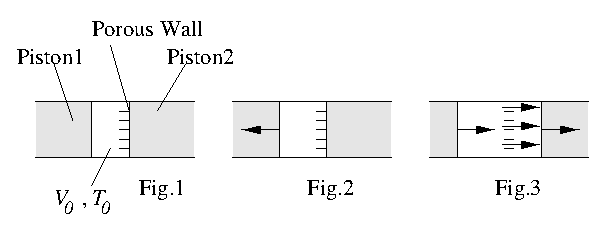
\includegraphics[clip]{1994phys-1.eps}}
  \end{center}

\end{subquestions}
\end{question}
\begin{answer}{教育 物理}{}

\begin{subanswers}
\SubAnswer

  \begin{subsubanswers}
  \SubSubAnswer
    地球の重力場から受ける力を代入するとロケットの運動方程式は次の
    ようになる。
%
    \begin{eqnarray}
      m\Bigl[\ddot{r}-r\dot{\theta}^2\Bigr] &=& F_r = -\frac{GMm}{r^2}
      \eqname{1-1} \\
      \Deriver{}{t} \Bigl[mr^2\dot{\theta}\Bigr] &=& rF_\theta = 0
      \eqname{1-2}
    \end{eqnarray}
%
    角運動量の $z$ 成分は $L_z=mr^2\dot{\theta}$ で表されるので、
    式\eqhref{1-2}から直ちに
%
    \[ mr^2\dot{\theta} = {\rm const} = L \]
%
    とわかる。$\dot{\theta}=L/mr^2$ を 
    式\eqhref{1-1}に代入して、$r$ 方向の運動方程式は
%
    \begin{equation}
      m \left( \ddot{r} - \frac{L^2}{m^2r^3} \right) = -\frac{GMm}{r^2}
      \eqname{1-3}
    \end{equation}
%
    と書き直される。

  \SubSubAnswer
    今、角運動量はゼロなので、式\eqhref{1-3}で $L=0$ とおいた式に
    両辺 $\dot{r}$ をかけて積分すると、$E$ を積分定数として
%
    \begin{equation}
      \frac{1}{2} m\dot{r}^2 - \frac{GMm}{r} = E \eqname{1-4}
    \end{equation}
%
    となる。$E$ がロケットの力学的エネルギーである。
    離脱速度 $v_1$ は上の式で$E=0,r=R$ とおいたときの $\dot{r}$ で
    ある。
%
    \[ v_1 = \sqrt{\frac{2GM}{R}}%
           =  \sqrt{\frac{2 \cdot 6.67\Keta{-11}\Unit{Nm^2kg^{-2}}
                \cdot 5.97\Keta{24} \Unit{kg} }
                {6.38\Keta{6}\Unit{m}}
              }%
           \simeq 1.12\Keta{4} \Unit{m/s} \]
%

  \SubSubAnswer
    離脱速度で発射するので式\eqhref{1-4}で $E=0$ であり、前問の
    $v_1$を用いると
%
    \[ \Deriver{r}{t} = v_1 \sqrt{\frac{R}{r}} \hspace{15mm}%
       \Yueni \d{t} = \frac{1}{v_1}\sqrt{\frac{r}{R}} \d{r} \]
%
    $r$が$R$から$4R$になるのにかかる時間 $t$は、
%
    \begin{eqnarray*}
      t &=& \int \d{t}%
         =  \Dint{R}{4R}{\d{r}} \frac{1}{v_1}\sqrt{\frac{r}{R}}%
         =  \frac{14}{3} \frac{R}{v_1} \\
        &=& \frac{14}{3} \times \frac{6.38\Keta{6}\Unit{m}}%
                                 {1.12\Keta{4} \Unit{m/s}}%
        \simeq 2700\Unit{sec}
    \end{eqnarray*}


  \SubSubAnswer
    円軌道なので
%
    \[ \dot{r}=\ddot{r}=0 \quad%
       r={\rm const} \quad%
       \dot{\theta}={\rm const}=\omega = 2\pi/T \]
%
    である。これらを式\eqhref{1-1}に代入して
%
    \[ T^2 = \frac{r^3 (2\pi)^2}{GM} \]
%
    を得る。\\
%
    特に、$r=4R$ のとき、
%
    \[ T = 2\pi \sqrt{\frac{(4R)^3}{GM}}%
         = 16\sqrt{2}\pi R \sqrt{\frac{R}{2GM}}%
         = 16\sqrt{2}\pi \frac{R}{v_1}%
         \simeq 40000 \Unit{sec} \simeq 11\Unit{hour} \]
%
    であるから、静止衛星の軌道は $4R$ 以上である。

  \end{subsubanswers}


\newpage
\SubAnswer
  磁場に関するアンペールの定理より
%
  \begin{equation}
     \oint \vec{H} \cdot \d{\vec{\ell}}%
     = \int_{S} \vec{i} \cdot \vec{n} \d{S} \eqname{2-1}
  \end{equation}
%
  であることを用いて各問を解く
 
  \begin{subsubanswers}
  \SubSubAnswer
    磁場の成分は明らかに $\phi$成分\,(直線電流を回る方向)\,$H_{\phi}$
    のみである。図1の平面で式\eqhref{2-1}を考えると、
%
    \[ 2\pi\rho H_{\phi} = -I \hspace{15mm}%
       \Yueni H_{\phi} = -\frac{I}{2\pi\rho} \]
%
    と求まる。

  \SubSubAnswer
    これも磁場の成分は$H_{\phi}$のみである。図2の2つの曲面でそれぞれ
    式\eqhref{2-1}を考える。角度$\theta$の立体角が
    $(1-\cos{\theta})/2$であることを考慮すると、上の曲面では
    直線電流が下へ流れ、放射電流が上へ流れるので
%
    \[  2\pi\rho H_{\phi} = -I+I\frac{1-\cos{\theta}}{2} \hspace{15mm}%
        \Yueni H_{\phi}=-\frac{I}{2\pi\rho}\frac{1+\cos{\theta}}{2} \]
%
    となり、下の曲面では放射電流が下へ流れるので
%
    \[  2\pi\rho H_{\phi}=-I\frac{1-\cos{(\pi-\theta)}}{2} \hspace{12mm}%
        \Yueni H_{\phi}=-\frac{I}{2\pi\rho}\frac{1+\cos{\theta}}{2} \]
%
    となり、結局どちらでも同じである。\\
%
    電流密度は デルタ関数とヘビサイド関数 $\theta(z)$ を用いて
%
    \[ \vec{i} = -I \delta(x)\delta(y)\theta(z) \vec{e}_z%
                 + \frac{I}{4\pi r^2}\vec{e}_r \]
%
    と表される。


  \SubSubAnswer
    $r=\infty$に極板を想定すれば、$z=0$の点電荷とコンデンサをなす。
    アンペールの定理はコンデンサ間の電場の変化を変位電流としてとらえる
    ことにより、普通にその間を電流が流れているとして扱うことができる。
    よってこの問題は設問(ii)と全く同じ状況となる。
%
    \[ H_{\phi} = -\frac{I}{2\pi\rho}\frac{1+\cos{\theta}}{2} \]
%

  \end{subsubanswers}

%
  \begin{center}
    \mbox{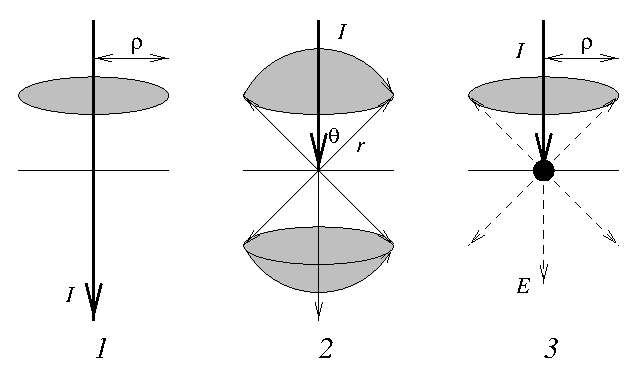
\includegraphics[clip]{1994phys-2.eps}}
  \end{center}

\newpage
\SubAnswer
  \begin{subsubanswers}
  \SubSubAnswer
    理想気体の断熱過程では、次のPoisson関係が成り立つ
%
    \[ TV^{\gamma-1} = {\rm Const} \hspace{1cm}%
       \gamma = \frac{C_p}{C_v}=\frac{5}{3} \]
%
    ここで、定積モル比熱$C_v=\frac{3}{2}R$、
    定圧モル比熱$C_p=\frac{5}{2}R$を用いた。
    上の関係式より、求める温度を$T_1$とすると
%
    \[ T_oV_o^{\frac{2}{3}} = T_1(8V_o)^{\frac{2}{3}} \hspace{1cm}%
       T_1 = \frac{T_o}{4} \]

  \SubSubAnswer
    下図のような膨張過程の際、気体は壁の左の領域から押し出されるときに
    ピストンより$p_1V_1$の仕事をされ、壁の右の領域に入る時には$p_2V_2$
    の仕事をピストン2にしている。その時気体の内部エネルギーの変化を考
    えると、
%
    \[ U_2 - U_1 = p_1V_1 - p_2V_2 \hspace{15mm}%
       \Yueni H_1 = U_1+p_1V_1 = U_2+p_2V_2 = H_2 \]
%
    よってエンタルピーは保存する。
%
    \begin{center}
      \mbox{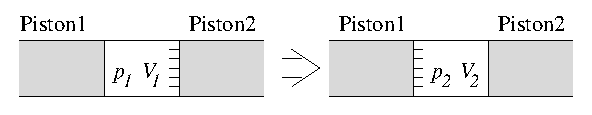
\includegraphics[clip]{1994phys-3.eps}}
    \end{center}


  \SubSubAnswer
    (ii)の過程は、始めと終りでエンタルピーが保存しているから、その
    温度変化は
%
    \[ T_2-T_1 = \Dint{p_1}{p_2}{\d{p}}%
                 \left(\Partial{T}{p}\right)_H \]
%
    で与えられる。この被積分関数は、Maxwellの関係式などより
%
    \[ \left(\Partial{T}{p}\right)_H%
       = -\left(\Partial{H}{p}\right)_T\left(\Partial{T}{H}\right)_p%
       ,\quad%
       \left(\Partial{H}{p}\right)_T%
       = -T\left(\Partial{V}{T}\right)_p+V%
       ,\quad%
       \left(\Partial{T}{H}\right)_p%
       =\left(\Partial{H}{T}\right)_p^{-1}=\frac{1}{C_p} \]
%
    すなわち、
%
    \begin{equation}
      \left(\Partial{T}{p}\right)_H%
      = \frac{1}{C_p}\left[T\left(\Partial{V}{T}\right)_p-V\right]%
      \eqname{3-1}
    \end{equation}
%
    で与えられる。今、気体を理想気体とすると、$pV=nRT$より
%
    \[ T\left(\Partial{V}{T}\right)_p-V = \frac{nRT}{p} - V = 0 \]
%
    よって、設問(ii)の過程で温度変化はなく、説問(i)で求めた温度
    $T_o/4$がこの過程を通じての気体の温度となる。


  \SubSubAnswer
    設問(iii)で求めた式\eqhref{3-1}に、気体の状態方程式
%
    \[ pV = nRT + Bp \]
%
    を代入すると
%
    \[ \left(\Partial{T}{p}\right)_H = -\frac{B}{C_p} \hspace{15mm}%
       \Yueni T = -\frac{B}{C_p}p+A  \qquad A={\rm const} \]
%
    を得る。設問(i)の結果より
%
    \[ \frac{T_o}{4} = -\frac{B}{C_p}p_1+A \quad\quad%
       p_1 = \frac{1}{32}p_o \]
%
    であったので、設問(ii)の過程の終状態における温度は、
%
    \[ T = -\frac{B}{C_p}\frac{p_1}{10}+A%
         = \frac{9}{320}\frac{B}{C_p}p_o+\frac{T_o}{4} \]
%
    となる。\\
%
    Bの正負によって、$\ds{\left(\Partial{T}{p}\right)_H}$
    の正負が決まり、よって、設問(i)の前後での温度の増減が定まる。


  \end{subsubanswers}
\end{subanswers}
\end{answer}


\end{document}
